\documentclass{article}

\usepackage[preprint]{neurips_2025}
\usepackage[utf8]{inputenc}
\usepackage[T1]{fontenc}
\usepackage{hyperref}
\hypersetup{hidelinks}
\usepackage{url}
\usepackage{booktabs}
\usepackage{amsmath}
\usepackage{amssymb}
\usepackage{microtype}
\usepackage{graphicx}
\usepackage{xcolor}
\usepackage{enumitem}

\definecolor{draftblue}{HTML}{2457A6}
\newcommand{\systemspec}{\textsc{SystemSpec}}
\newcommand{\suto}{\textsc{Suto}}
\newcommand{\code}[1]{\texttt{#1}}

\title{Objective-Conditioned Black-Box Optimization\\of Simulated Scientific Institutions\\\large Science Utopia Lab --- Working Draft}

\author{Science Utopia Lab \\
\texttt{https://github.com/unktok/science-utopia-lab} \\
\textcolor{draftblue}{Authorship and affiliations to be finalized}}

\begin{document}

\maketitle

\begin{abstract}
Prior simulation studies of science compare interventions chosen in advance. We study a different problem: given an explicit objective, can a black-box optimizer search over the institution itself, and how does changing that objective alter the search path and the system selected? Science Utopia Lab extends the \suto{} closed-loop LLM-agent simulator with a versioned design object, a persistent \code{ask}/\code{tell} loop, and strict separation among optimization loss, technical validity, held-out evaluation, and post-evaluation policy. In a preregistered Qwen3-8B study, we hold the simulator, eight-parameter design space, optimizer, budget, and seeds fixed while changing only the loss. Three objectives each evaluate five candidate systems on three common development seeds, producing 45 terminal logical rows. They select two distinct designs, sealed before 15 common held-out runs. Cross-scoring the frozen designs yields a descriptive loss-dependent rank reversal, although all nine paired contrasts have 95\% intervals containing zero. The study therefore demonstrates objective-conditioned institutional search, not stable superiority, optimizer efficiency, structural optimization, or a real-world policy optimum. The broader framework represents evaluation, publication, funding, governance, communication, and other mechanisms as a typed \systemspec{} graph, making whole-system optimization the research target while clearly marking the current fixed-topology experiment as its first restricted slice.
\end{abstract}

\section{Introduction}

Science policy often asks a systems question: which institutional arrangements best support reliable, useful, diverse, and sustainable science? Real-world controlled experimentation is limited by cost, time, ethics, and the absence of counterfactual outcomes. Agent-based simulation can provide a laboratory for such questions, but comparison of hand-selected interventions is only the first step. If a complete simulated scientific ecosystem is viewed as a stochastic function, institutional design becomes an optimization problem: the objective is chosen explicitly, while the institution is the variable to be searched.

The original \suto{} framework models persistent researchers, institutions, funding, collaboration, submission, peer review, resubmission, citation, and attrition across simulated years~\citep{jin2026scienceutopia}. Its 61 reported worlds compare investigator-specified strategies and institutional interventions, including exploration behavior, resubmission, selectivity, disclosure, and funding capacity. Those experiments ask what happens under a chosen condition. Science Utopia Lab starts from the same simulator but asks a different methodological question: conditional on a declared objective, what \emph{system that organizes science} does a sequential optimizer discover?

\begin{table}[t]
\caption{The base simulator and Science Utopia Lab use related machinery but different experimental objects.}
\label{tab:suto-vs-lab}
\centering
\small
\begin{tabular}{p{0.18\linewidth}p{0.36\linewidth}p{0.36\linewidth}}
\toprule
 & Original \suto{} studies & Science Utopia Lab \\
\midrule
Intervention & Hand-specified strategy or institutional condition & Versioned optimization objective \\
Variable of interest & Outcomes under fixed conditions & Search path and resulting \systemspec{} \\
Feedback & Within-world scientific dynamics & Within-world dynamics plus optimizer \code{tell}$\rightarrow$\code{ask} \\
Primary evidence & Matched counterfactual effects & Objective-conditioned trajectories, selected systems, and cross-objective held-out behavior \\
\bottomrule
\end{tabular}
\end{table}

This distinction matters. Reporting that one acceptance rate or funding rule changes an outcome would largely repeat the intervention logic already enabled by \suto{}. Our object of study is instead the map
\begin{equation}
    \text{objective} \longrightarrow \text{search trajectory} \longrightarrow \text{selected institution} \longrightarrow \text{held-out profile}.
\end{equation}
The central scientific questions are therefore whether objectives induce different search paths, whether those paths select different systems, and what trade-offs appear when every frozen system is scored under every objective. A later question is whether one optimizer reaches better systems per simulation budget than another.

This problem is deceptively difficult. A scalar objective can turn an observable proxy into an unintended target, a problem closely related to Campbell's law and metric gaming~\citep{campbell1979assessing,fire2019overoptimization}. Technical failures must not be silently converted into bad objective values. Metrics used during search cannot simultaneously be described as held out. Finally, optimizing only a peer-review parameter would mistake one mechanism for the entire scientific institution.

This report makes four contributions:

\begin{enumerate}[leftmargin=*,nosep]
    \item an objective-conditioned research design in which the loss, rather than a hand-selected institution, is the experimental intervention;
    \item a persistent black-box loop that records how observations generate later system proposals and keeps loss, validity, held-out metrics, and decision policy separate;
    \item a first equal-budget, three-objective experiment with frozen winners and complete cross-objective held-out scoring; and
    \item a typed whole-system representation that extends the design target beyond peer review while refusing to describe the current fixed-topology runtime as structural optimization.
\end{enumerate}

The empirical contribution is intentionally narrow. We hold the simulator, design space, search budget, and seeds fixed while changing only the optimized loss. This isolates the first link in the map above, but the five-candidate budget, frequent technical invalidity, and two distinct winners do not yet support a strong claim about optimizer efficiency or path diversity. The common held-out split completed with no technical failure and entered this draft through an atomic completion gate. We do not claim that any proxy measures scientific value or that a selected candidate should inform real policy.

\section{Problem Formulation}

Let $S$ denote a complete specification of a scientific institution, $c$ an environmental context, and $\xi$ stochasticity including simulator seeds and model sampling. A simulator produces a trajectory
\begin{equation}
    \tau \sim \mathrm{Sim}(S,c,\xi),
\end{equation}
containing agent states, scientific artifacts, decisions, resource transfers, and events over time. An optimization loss $L$ maps replicated trajectories to a scalar used by a search algorithm:
\begin{equation}
    S_{t+1} \sim \mathcal{A}\!\left(\{S_i,L(S_i)\}_{i=1}^{t}\right).
\end{equation}
Here $\mathcal{A}$ may be random search, Bayesian optimization, an evolutionary method, or a differentiable procedure over a relaxation of $S$. The simulator remains opaque to the generic \code{ask}/\code{tell} interface.

\subsection{The system, not peer review, is the design object}

We represent $S$ as a \systemspec{} containing agent and artifact types, mechanism instances, typed input/output ports, directed connections, schedules, initial state, invariants, and metadata. Mechanism families may include research, evaluation, publication, funding, governance, communication, collaboration, employment, and education. No family---including evaluation---is structurally mandatory. A publication-only or even empty graph is valid when its declared ports and invariants are satisfied.

The present implementation can describe general typed graphs but executes a restricted subspace through a strict legacy compiler. The compiler accepts the known fixed topology and refuses unsupported node addition, removal, or substitution. This refusal is important: structural freedom in a schema is not yet structural freedom in the runtime. The next runtime milestone is an implementation registry and generic graph executor.

\subsection{Four contracts that must remain separate}

We use the machine-learning analogy of training loss and held-out accuracy while making the split explicit (Table~\ref{tab:contracts}). Technical validity only determines whether a run yields an admissible observation. It does not impose an unrecorded ethical or distributional veto. Conversely, a held-out metric ceases to be held out once it influences proposals or candidate selection.

\begin{table}[t]
\caption{Distinct roles in an auditable optimization campaign.}
\label{tab:contracts}
\centering
\small
\begin{tabular}{p{0.23\linewidth}p{0.43\linewidth}c}
\toprule
Contract & Role & Search-visible? \\
\midrule
\code{LossSpec} & Scalar or vector directly optimized on declared seeds & Yes \\
\code{ValiditySpec} & Completion, schema, accounting, and provenance checks & Admissibility only \\
Evaluation metric spec & Held-out performance, robustness, slices, and uncertainty & No \\
\code{DecisionPolicy} & Optional post-evaluation promotion or deployment rule & No \\
\bottomrule
\end{tabular}
\end{table}

This architecture avoids a previous failure mode in institutional comparison: adding substantive floors or protected-slice vetoes outside the declared objective. Such rules can be valuable, but only as explicit, versioned constraints or post-evaluation policies. They are not implicit defaults.

% Method boundary, intentionally independent of experimental result values.
\begin{figure}[t]
\centering
\setlength{\fboxsep}{5pt}
\begin{minipage}{0.98\linewidth}
\small
\centering
\textbf{Objective is the intervention; the institution is the search output}

\vspace{4pt}
\begin{tabular}{ccc}
\fbox{\parbox{0.27\linewidth}{\centering
\textbf{LossSpec A}\\participation $+$ review\\
$\downarrow$\\search path A $\rightarrow S_A^*$}}
&
\fbox{\parbox{0.27\linewidth}{\centering
\textbf{LossSpec B}\\topic-entropy proxy\\
$\downarrow$\\search path B $\rightarrow S_B^*$}}
&
\fbox{\parbox{0.27\linewidth}{\centering
\textbf{LossSpec C}\\review-burden proxy\\
$\downarrow$\\search path C $\rightarrow S_C^*$}}
\end{tabular}

\vspace{5pt}
Each path repeats: \code{ask} $\rightarrow$ candidate \systemspec{}
$\rightarrow$ development simulation $\rightarrow$ \code{ValiditySpec}
$\rightarrow$ declared loss $\rightarrow$ \code{tell}.

\vspace{4pt}
$\Downarrow$ simultaneous immutable winner freeze $\Downarrow$

\vspace{4pt}
\fbox{\begin{minipage}{0.92\linewidth}
\centering
\textbf{Common held-out cross-evaluation}\quad
$\{S_A^*,S_B^*,S_C^*\}\times$ untouched seeds $\times$
$\{L_A,L_B,L_C,\text{diagnostics}\}$

\smallskip
rank reversals $+$ uncertainty $+$ trade-offs $+$ gaming diagnostics
\end{minipage}}

\vspace{3pt}
Held-out results never return to \code{ask}; an optional
\code{DecisionPolicy} remains separately versioned.
\end{minipage}
\caption{Central experimental logic. Unlike a fixed intervention comparison,
the objective conditions the sequential process that produces each institution.
Loss, technical validity, held-out evaluation, and post-evaluation policy remain
distinct contracts.}
\label{fig:metric-conditioned-methods-flow}
\end{figure}


\section{System Architecture}

The implemented loop is summarized below:

\begin{center}
\fbox{\begin{minipage}{0.92\linewidth}
\centering
\code{optimizer.ask()} $\rightarrow$ versioned \systemspec{} $\rightarrow$ seed-replicated simulator jobs\\
$\downarrow$ \hfill canonical events, snapshots, hashes \hfill $\downarrow$\\
\code{optimizer.tell(observation)} $\leftarrow$ \code{LossSpec} aggregation $\leftarrow$ \code{ValiditySpec}
\end{minipage}}
\end{center}

\paragraph{Opaque optimizer boundary.} A search-space adapter is the only component that understands candidate structure. The optimizer receives JSON-compatible system objects and finite loss observations; it does not import simulator internals, held-out metrics, or a promotion policy. The baseline \code{AdaptiveRandomSearch} first emits deterministic independent points, then mutates the lowest-loss incumbent after observations are returned. Pending suggestions, observations, and proposal state are serialized.

\paragraph{Persistent campaign controller.} Each suggestion is persisted before dispatch. The controller registers one job per optimization seed, records attempts and provenance, aggregates only technically valid runs, and checkpoints optimizer state. Restart tests require state, snapshot, registry, loss reports, and rendered status to remain byte-stable when no new work occurs.

\paragraph{Canonical event replay.} Simulator outputs are converted into a versioned event stream and deterministically projected into state. The same authoritative replay artifact supplies audit views and the game UI. This makes the interface a view over evidence rather than a second, divergent simulation.

\paragraph{Reproducibility boundary.} Campaign files pin the source revision, model and backend, loss hash, search seed, optimization and held-out seed sets, fidelity, worker count, and suggestion budget. Raw model caches and large outputs remain outside Git; compact results, hashes, protocols, and interpretation are versioned.

% Result insertion boundary for the preregistered metric-conditioned study.
% The graphics CLI refuses to place synthetic fixtures in this directory.
\newif\ifmetricconditionedresults
\metricconditionedresultsfalse
\IfFileExists{figures/metric-conditioned/metric-conditioned-cross-evaluation.pdf}{%
  \IfFileExists{figures/metric-conditioned/metric-conditioned-objective-trajectories.pdf}{%
    \IfFileExists{figures/metric-conditioned/metric-conditioned-tradeoff-rank-generalization.pdf}{%
      \metricconditionedresultstrue
    }{}%
  }{}%
}{}

\section{Metric-Conditioned Optimization Study}
\label{sec:metric-conditioned-results}

The preregistered study holds the design space, optimizer, budget, and seeds
fixed while changing only the optimization loss. Each arm freezes its winner
before a common held-out suite evaluates all three systems. Topic entropy and
review burden are deliberately narrow proxy objectives, not normative policy
recommendations. This section reports results only when the complete,
experiment-classified three-figure set is present.

\ifmetricconditionedresults
\begin{figure}[t]
    \centering
    \includegraphics[width=0.92\linewidth]{figures/metric-conditioned/metric-conditioned-cross-evaluation.pdf}
    \caption{Cross-evaluation of the three frozen systems. Cell annotations are
    held-out losses in their native units; color encodes rank within each loss
    column, because losses are not commensurate across columns. Lower is better.}
    \label{fig:metric-conditioned-cross-evaluation}
\end{figure}

\begin{figure}[t]
    \centering
    \includegraphics[width=\linewidth]{figures/metric-conditioned/metric-conditioned-objective-trajectories.pdf}
    \caption{Arm-specific development trajectories. Points are observed losses,
    steps are incumbent losses, and stars mark frozen winners. Panels retain
    each objective's native units rather than implying that values are
    comparable across objectives.}
    \label{fig:metric-conditioned-trajectories}
\end{figure}

\begin{figure}[t]
    \centering
    \includegraphics[width=\linewidth]{figures/metric-conditioned/metric-conditioned-tradeoff-rank-generalization.pdf}
    \caption{Held-out trade-off, rank reversal, and generalization diagnostics
    for the frozen systems. These diagnostics characterize how the chosen loss
    changes the system found; they do not establish a universally best system.}
    \label{fig:metric-conditioned-diagnostics}
\end{figure}
\else
\begin{center}
\fbox{\parbox{0.9\linewidth}{\small\textbf{Result boundary.}
The metric-conditioned optimization and common held-out evaluation are not yet
complete in this source tree. No synthetic fixture or preliminary profile is
shown as an experimental result.}}
\end{center}
\fi


\section{Objectives as a Science-of-Science Problem}

The hard research problem is not merely selecting an optimizer; it is deciding what counts as a good scientific system. Science-of-science research characterizes funding, collaboration, careers, publication, and diffusion, but descriptive regularities do not automatically define normative objectives~\citep{fortunato2018science}. The Leiden Manifesto likewise argues that quantitative evaluation should support, not replace, expert judgment and should be matched to institutional missions~\citep{hicks2015leiden}.

Accordingly, future campaigns should retain a multi-dimensional measurement layer even if a temporary scalar is used during search. Candidate constructs include epistemic reliability and correction, useful exploration, diversity as variety/balance/disparity~\citep{stirling2007general}, resource efficiency, sustainable research capacity, distributional outcomes, public or mission value, and resistance to gaming. Reproducibility and replicability should remain distinct~\citep{nasem2019reproducibility}. Citation counts, publication counts, acceptance rates, and LLM review scores are diagnostics or proxies, not direct measurements of truth or social value.

This framing also clarifies the analogy with national science policy. Governments are important funders, rule setters, and beneficiaries, but their utility is not the sole welfare function. Researchers, affected communities, the international knowledge commons, future generations, and the environment can bear different benefits and burdens. Science Utopia should make those principals and trade-offs inspectable rather than hide them in one score.

\section{Related Work}

Our base simulator is \suto{}~\citep{jin2026scienceutopia}. Its matched counterfactuals vary investigator-selected strategies or institutional conditions and analyze their downstream effects. We instead intervene on the objective and study the search process that produces an institution. This complements rather than reproduces the original analyses: \suto{} supplies the longitudinal world, while Science Utopia Lab adds an outer optimization loop and makes objective-conditioned system discovery the experimental object.

Generative-agent systems have demonstrated persistent memory, reflection, and social interaction in simulated environments~\citep{park2023generative}, while \suto{} specializes these ideas to research ecosystems grounded in scientific artifacts. Black-box optimization provides methods for expensive, derivative-free objectives, including Bayesian optimization and evolutionary strategies~\citep{shahriari2016taking}. Our contribution is not a new optimizer or evidence that the present baseline is efficient. It is an interchangeable, auditable boundary through which optimizer methods can later be compared under equal simulation budgets.

Research assessment scholarship motivates the explicit separation between measured proxies and institutional goals. Campbell~\citep{campbell1979assessing} and later empirical work on academic metrics~\citep{fire2019overoptimization} warn that optimization pressure can change the process being measured. We therefore treat metric gaming as a future object of simulation, not merely measurement noise.

\section{Limitations, Risks, and Ethics}

\paragraph{Simulator validity.} An LLM-agent world is not a validated causal model of real academia. Results can reflect prompting, model priors, retrieval data, simplified resource accounting, or omitted mechanisms. Policy claims require external validation and sensitivity analysis beyond software correctness.

\paragraph{Objective misspecification.} The demonstrated objectives are coarse and normatively incomplete. Optimizing them at scale could reward survival without knowledge quality, maximize entropy without epistemic value, or reduce review burden by suppressing valuable evaluation. The two narrow proxy objectives selected the same design, and the diagnostic gaming flags show why proxy-specific improvements must not be treated as welfare improvements.

\paragraph{Restricted action space.} The optimizer currently mutates eight parameters within a fixed legacy topology. Although \systemspec{} can describe arbitrary mechanism graphs, the general executor and topology mutation operators are not yet implemented. We therefore do not claim structural optimization.

\paragraph{Sparse paths and no optimizer baseline.} The study has five proposals per arm. Two arms have only two technically valid designs and therefore provide little adaptive-path evidence. No equal-budget random, Sobol, Bayesian, or evolutionary baseline was run, and no optimizer-seed replication was performed. The experiment demonstrates a functioning objective-conditioned loop, not search efficiency or optimizer superiority.

\paragraph{Scale and uncertainty.} The engineering demonstration uses three one-year smoke worlds, and the objective-conditioned study uses three four-year development worlds per system plus five common held-out seeds. Every one of the nine paired held-out loss intervals contains zero, so the observed rank reversal is descriptive rather than evidence of stable pairwise superiority. Topic entropy and review burden also selected the same design; their separately simulated arm-labelled trajectories are stochastic repetitions, not distinct institutions. None of these simulations supports inference about real institutional effects.

\paragraph{Representational and governance risks.} Synthetic agents should not be assigned real protected characteristics by inference from names or text. Future fairness experiments should use explicit synthetic attributes and document causal assumptions. Human oversight, appeal, public legitimacy, scientific freedom, and externalized harms must remain visible when governance mechanisms are introduced.

\section{Roadmap}

The next research stage has four parallel tracks. First, replicate objective-conditioned paths with larger valid budgets, multiple optimizer seeds, design-collapsed analysis, and broader objective families. Second, compare random, Sobol, Bayesian, and evolutionary methods under an equal simulation budget, reporting incumbent loss versus evaluations rather than only final winners. Third, bind the existing mechanism registry and joint structural grammar into a sealed simulator-backed campaign so that evaluation, publication, funding, governance, and communication can be added, removed, or replaced. Fourth, investigate differentiable surrogates and connect the replay observatory to provenance-linked views of objective, path, system, and held-out evidence.

\section{Conclusion}

Science Utopia Lab turns institutional design into an explicit computational object. Its present empirical claim is specific: changing the optimized proxy can change the trajectory and frozen institutional design under otherwise common search conditions, and the resulting systems can exchange rank when cross-scored under different losses. This is conceptually different from comparing interventions chosen in advance, because the objective conditions the search that produces the intervention. It is also only a first slice: two objectives collapsed to the same design, invalid proposals truncated two adaptive paths, and five held-out seeds did not establish stable pairwise superiority. The next experiments must replicate optimizer paths, compare search methods under equal budgets, broaden objective families, and move from eight fixed-topology parameters toward mechanism structure.

\appendix

\section{Engineering Validation of the Result-Dependent Loop}

Before the objective-conditioned study, a separate campaign verified that a real simulator observation could change a later proposal. The campaign was frozen as \code{first-closed-loop-engineering} at revision \code{9a10029807d5}. It used Qwen3-8B through Ollama, smoke fidelity, one worker, and development seeds 503, 509, and 521. The restricted eight-parameter space matched the later study.

For run $r$, the engineering loss was $\ell_r=1-a_r+0.05b_r$, where $a_r$ is active-researcher fraction and $b_r$ is review burden per active researcher. The aggregate was $L(S)=\operatorname{mean}_r(\ell_r)+0.25\operatorname{sd}_{\mathrm{pop},r}(\ell_r)$. This was an infrastructure probe, not a scientific-quality or policy objective.

\begin{table}[h]
\caption{Engineering trace showing one observation-dependent proposal. Lower loss is better.}
\label{tab:engineering-trace}
\centering
\small
\begin{tabular}{llllr}
\toprule
Suggestion & Phase & Design & Parent observation & Loss \\
\midrule
\code{s48505e...} & Initial & \code{d0cff50...} & --- & 0.673379 \\
\code{s5aad19d...} & Initial & \code{d818522...} & --- & 0.421179 \\
\code{s78f27e...} & Adaptive & \code{d7e65ef...} & \code{o27437d...} & 0.421179 \\
\bottomrule
\end{tabular}
\end{table}

The adaptive design changed acceptance rate, funding-budget slot fraction, and resubmission cost, yet tied the incumbent on all three seeds. Thus the test establishes result dependence, not improvement. All nine runs completed and the campaign consumed 9,821.6 serial seconds. A separate four-worker microbenchmark against one local Ollama endpoint produced no material throughput gain, motivating independent inference endpoints for future replicated campaigns.

\section{Canonical Replay and Research Observatory}

Long-running multi-agent simulations are difficult to inspect from aggregate tables alone. The accompanying interface presents commit-pinned canonical event replay as a cyberpunk pixel-art research arcology (Figure~\ref{fig:game}). Users can step through time, follow researchers and institutional flows, and inspect evidence without treating presentation-only choreography as simulation output.

\begin{figure}[h]
    \centering
    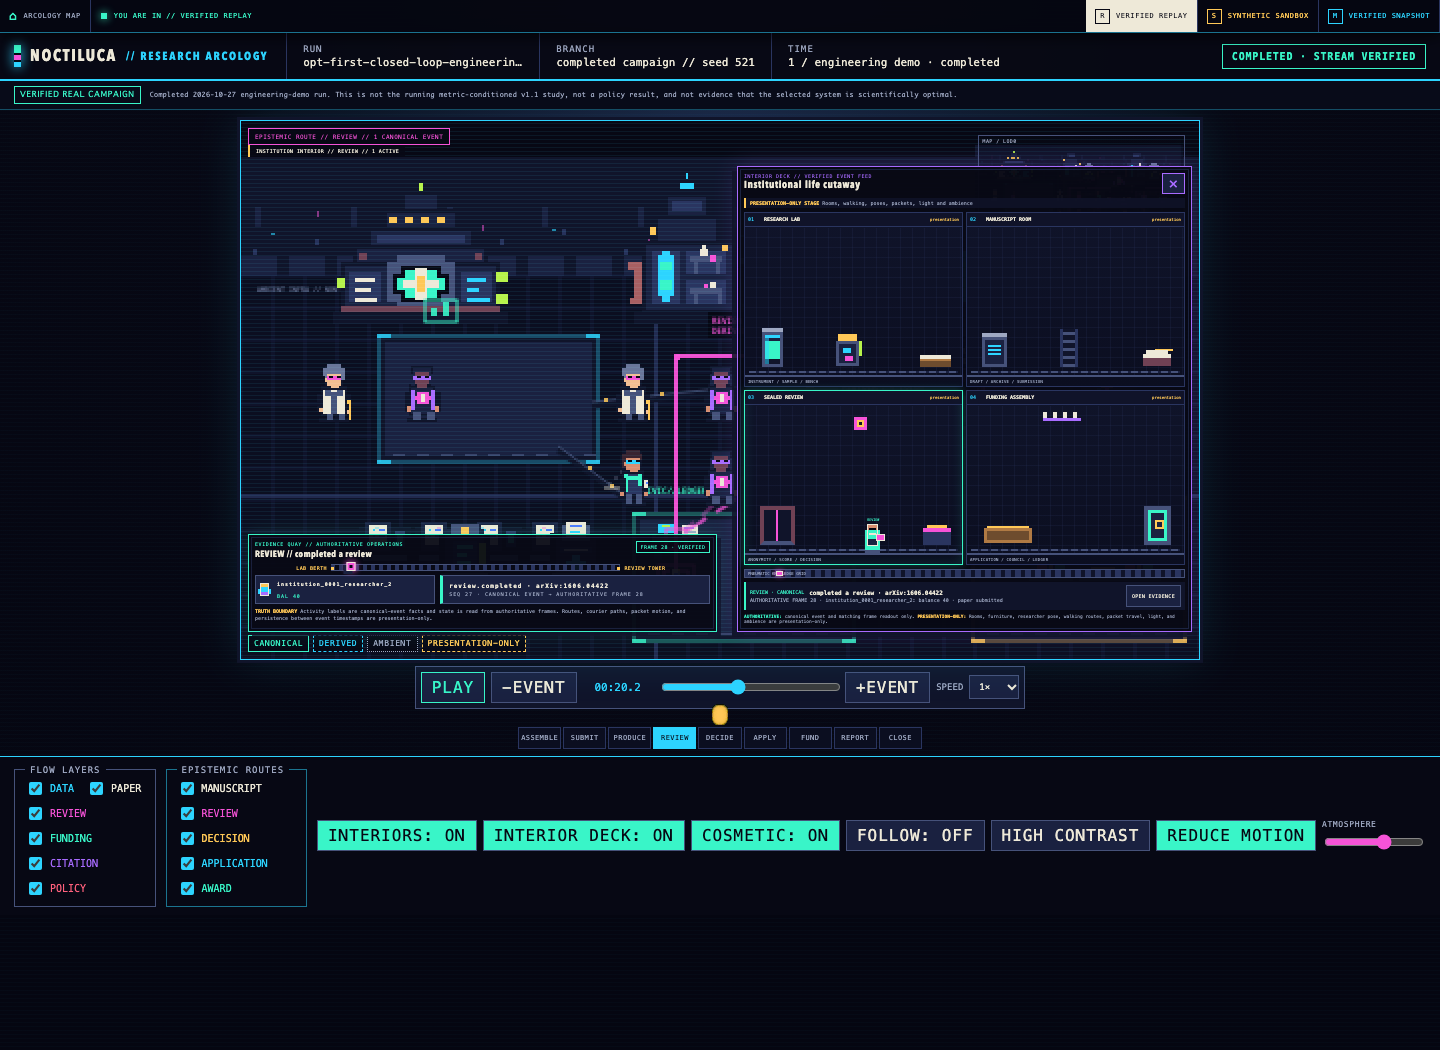
\includegraphics[width=0.92\linewidth]{figures/game-ui.png}
    \caption{Real-browser capture of a verified seed-521 peer-review event. Event identity and authoritative frame are grounded in commit-pinned replay; room layout, poses, packet motion, and lighting are presentation-only. This engineering campaign is not evidence from the objective-conditioned study.}
    \label{fig:game}
\end{figure}

The verified replay remains read only: an intervention creates a new, versioned branch rather than mutating recorded history. This interface is supporting research infrastructure, not a contribution to the optimization result itself.

\section*{Reproducibility Statement}

The repository contains campaign protocols, loss specifications, design-space schemas, compact machine-readable results, artifact hashes, tests, figure-generation code, and UI source. The first closed-loop result records revision \code{9a10029807d5}. The metric-conditioned optimization used clean source commit \code{1078279d1ce833afe9ffb6b7c262da15357b76ab}, study revision \code{23cbe8a107e5}, and protocol tag \code{protocol/metric-conditioned-optimization-v1.1}; its three-winner freeze hash is \code{254c3366e921...}. The commit-pinned cross-evaluation report and independently validated paper slice are hash-recorded in the generated artifact manifest. Large raw outputs remain at their recorded locators and are intentionally not committed.

\bibliographystyle{plainnat}
\bibliography{references}

\end{document}
